\FloatBarrier
\subsection{RLS \& ELS identification with Colored noise on output}
The system input for this section was white noise with a variance of $2$. The Simulink model used was consistent with that shown in \autoref{fig:LSICNOSimulinkModel}. The comparison between the actual and RLS-identified system outputs is presented in \autoref{fig:RLSICNOWhiteNoiseOutput}. The parameter evaluation is depicted in \autoref{fig:RLSICNOWhiteNoiseParams}, and the derived transfer function for the system with colored output noise is given in \autoref{eq:RLSICNOTransferFunction}.
  
\begin{figure}
	\centering
	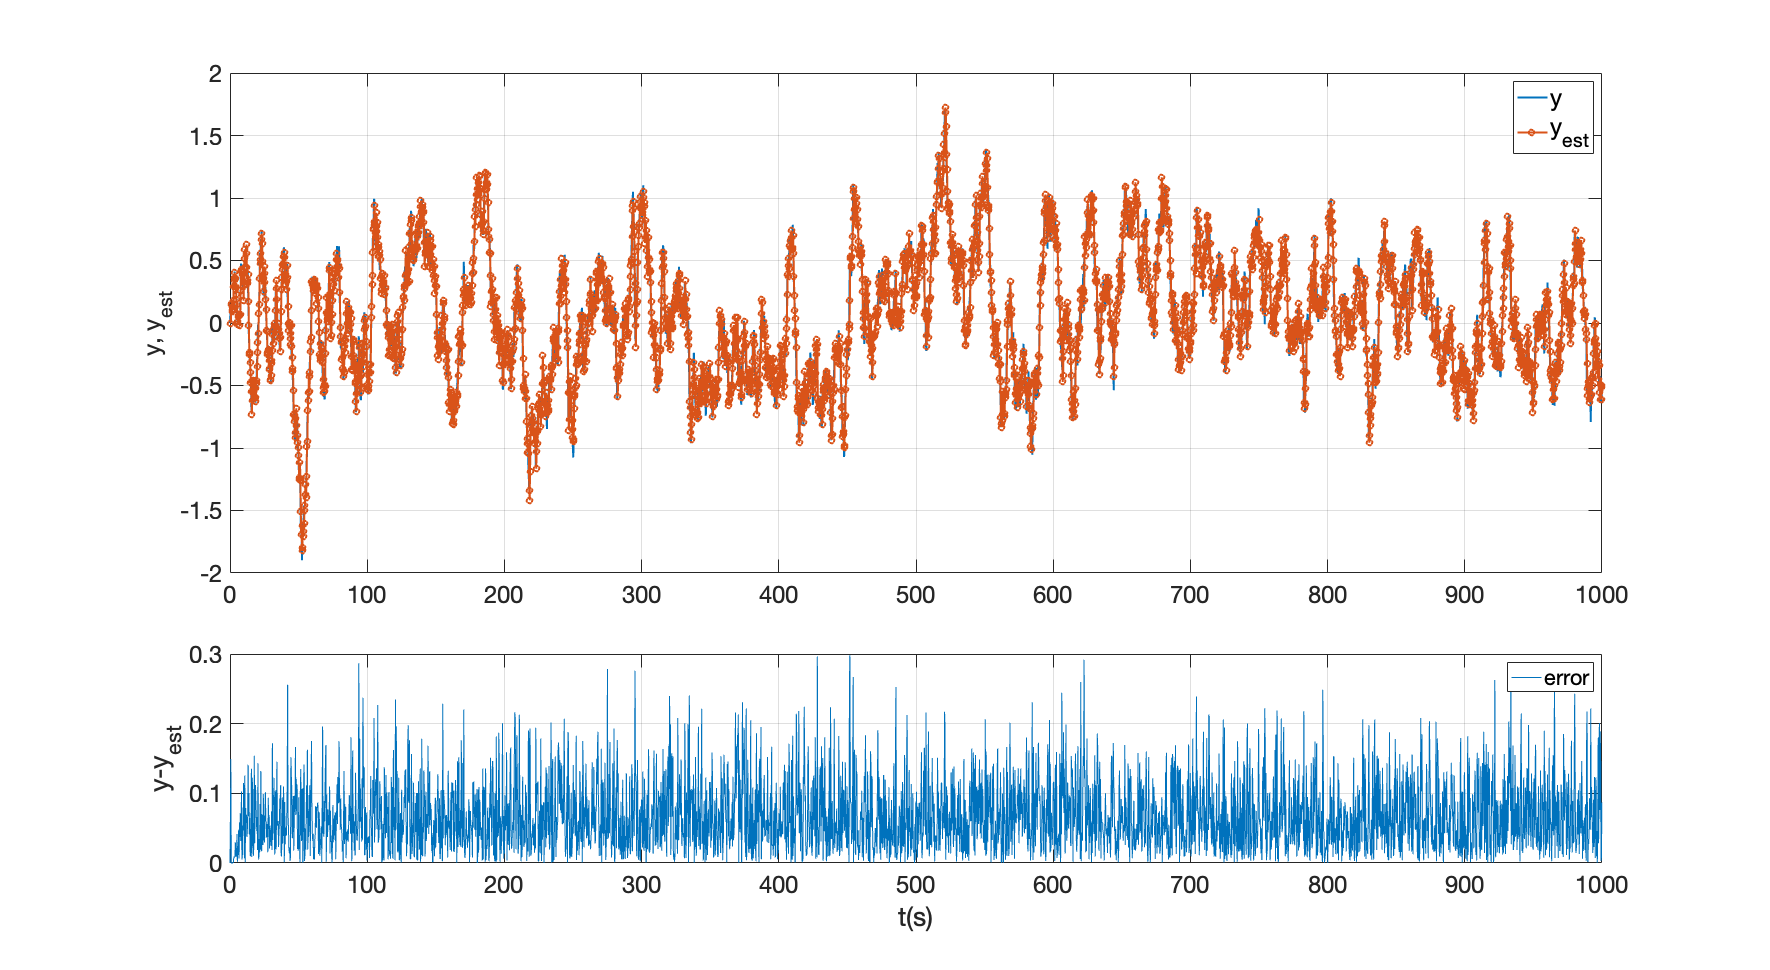
\includegraphics[totalheight=8cm]{images/RLSICNOWhiteNoiseOutput.png}
	\caption{RLS system output comparison for colored noised on output}
	\label{fig:RLSICNOWhiteNoiseOutput}
\end{figure}

\begin{figure}
	\centering
	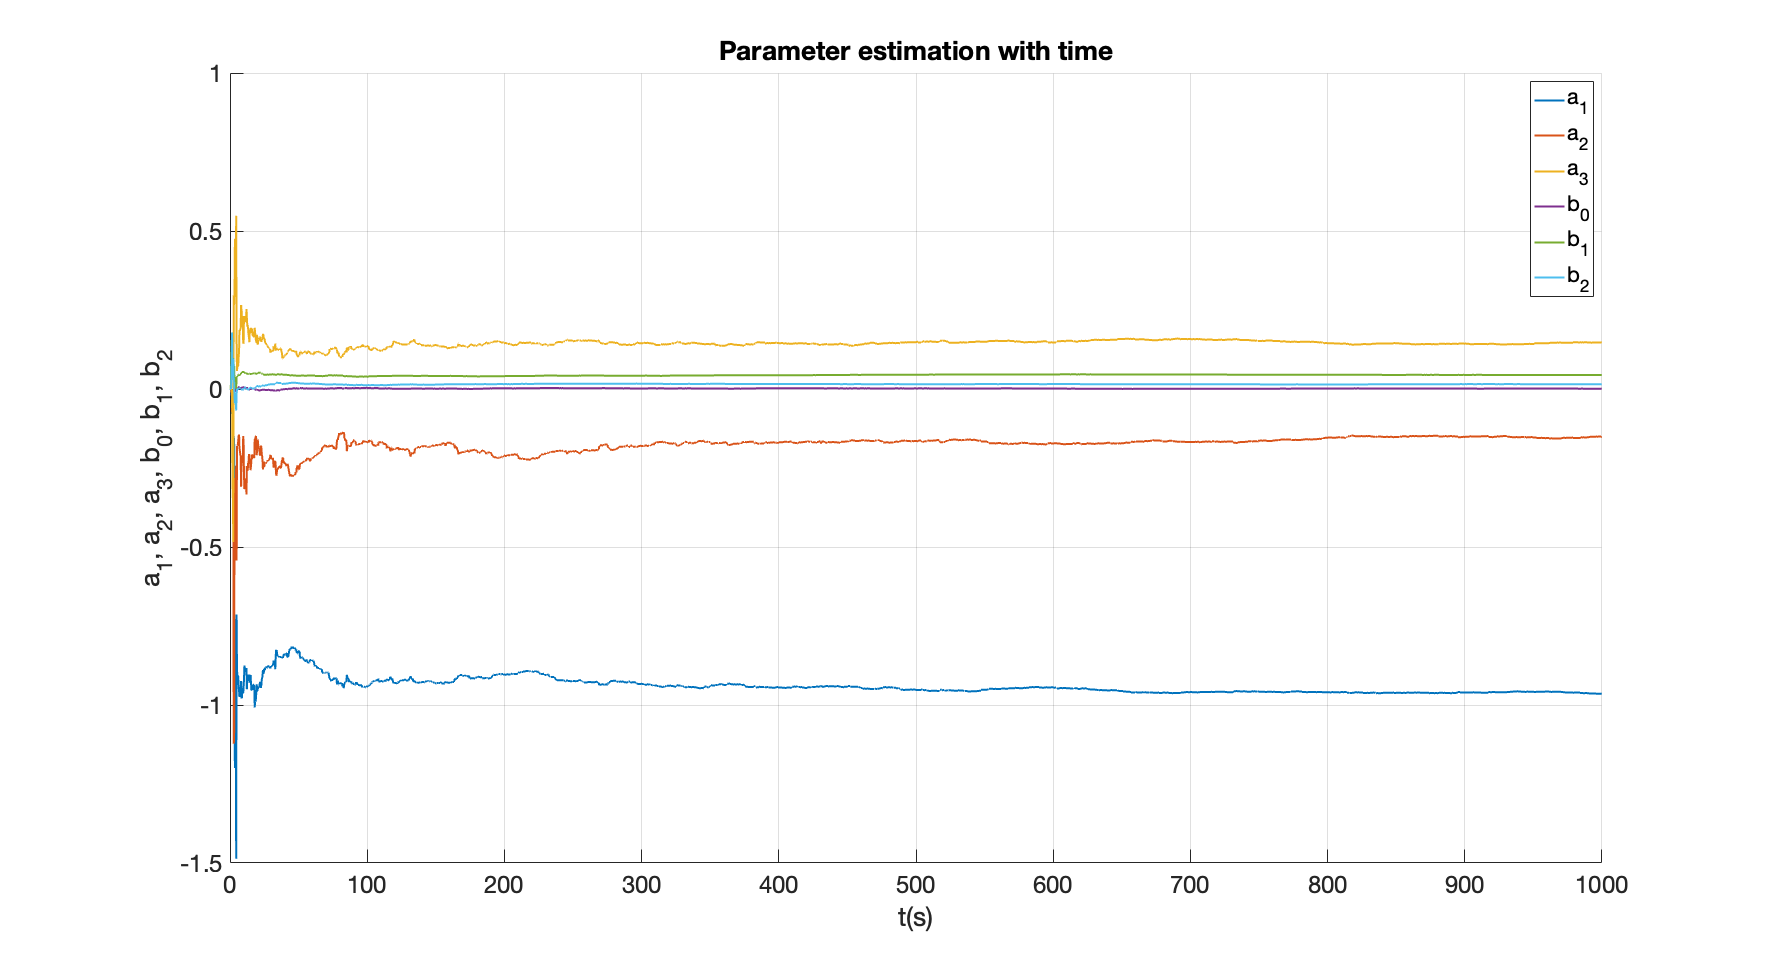
\includegraphics[totalheight=8cm]{images/RLSICNOWhiteNoiseParams.png}
	\caption{RLS system parameters with colored noise on output}
	\label{fig:RLSICNOWhiteNoiseParams}
\end{figure}

\begin{equation}
	G(z) =	\frac{ -0.001275 z^2 + 0.04381 z + 0.01426}{z^3 - 0.9867 z^2 - 0.07868 z + 0.09777}
	\label{eq:RLSICNOTransferFunction}
\end{equation}

The Simulink model for RLS identification with colored noise on output can be accessed at \hspace{-1ex}\lstinline| assignment1/part2/2_4/RLS2_4_clrd.slx|.
Matlab code for system is at \hspace{-1ex}\lstinline| assignment1/part2/2_2/RLS2_4_colored.m|.

The Matlab implementation of the ELS\footnote{Extended Least Squares } is provided and can be accessed at \hspace{-1ex}\lstinline| assignment1/part2/2_4/RLS2_4_colored_ELS.m|.
\autoref{fig:ELSIColoredNoiseOutput} shows the comparison between the outputs of the actual system and identified one using the ELS. \autopageref{fig:ELSISystemParam} presents the evaluation of system parameters.
The parameters of the noise is calculated in each cycle and \autopageref{fig:ELSINoiseParam} presents them. The transfer function of the identified system using ELS with colored noise on output is available at \autoref{eq:ELSITransferFunction}.

\begin{figure}
	\centering
	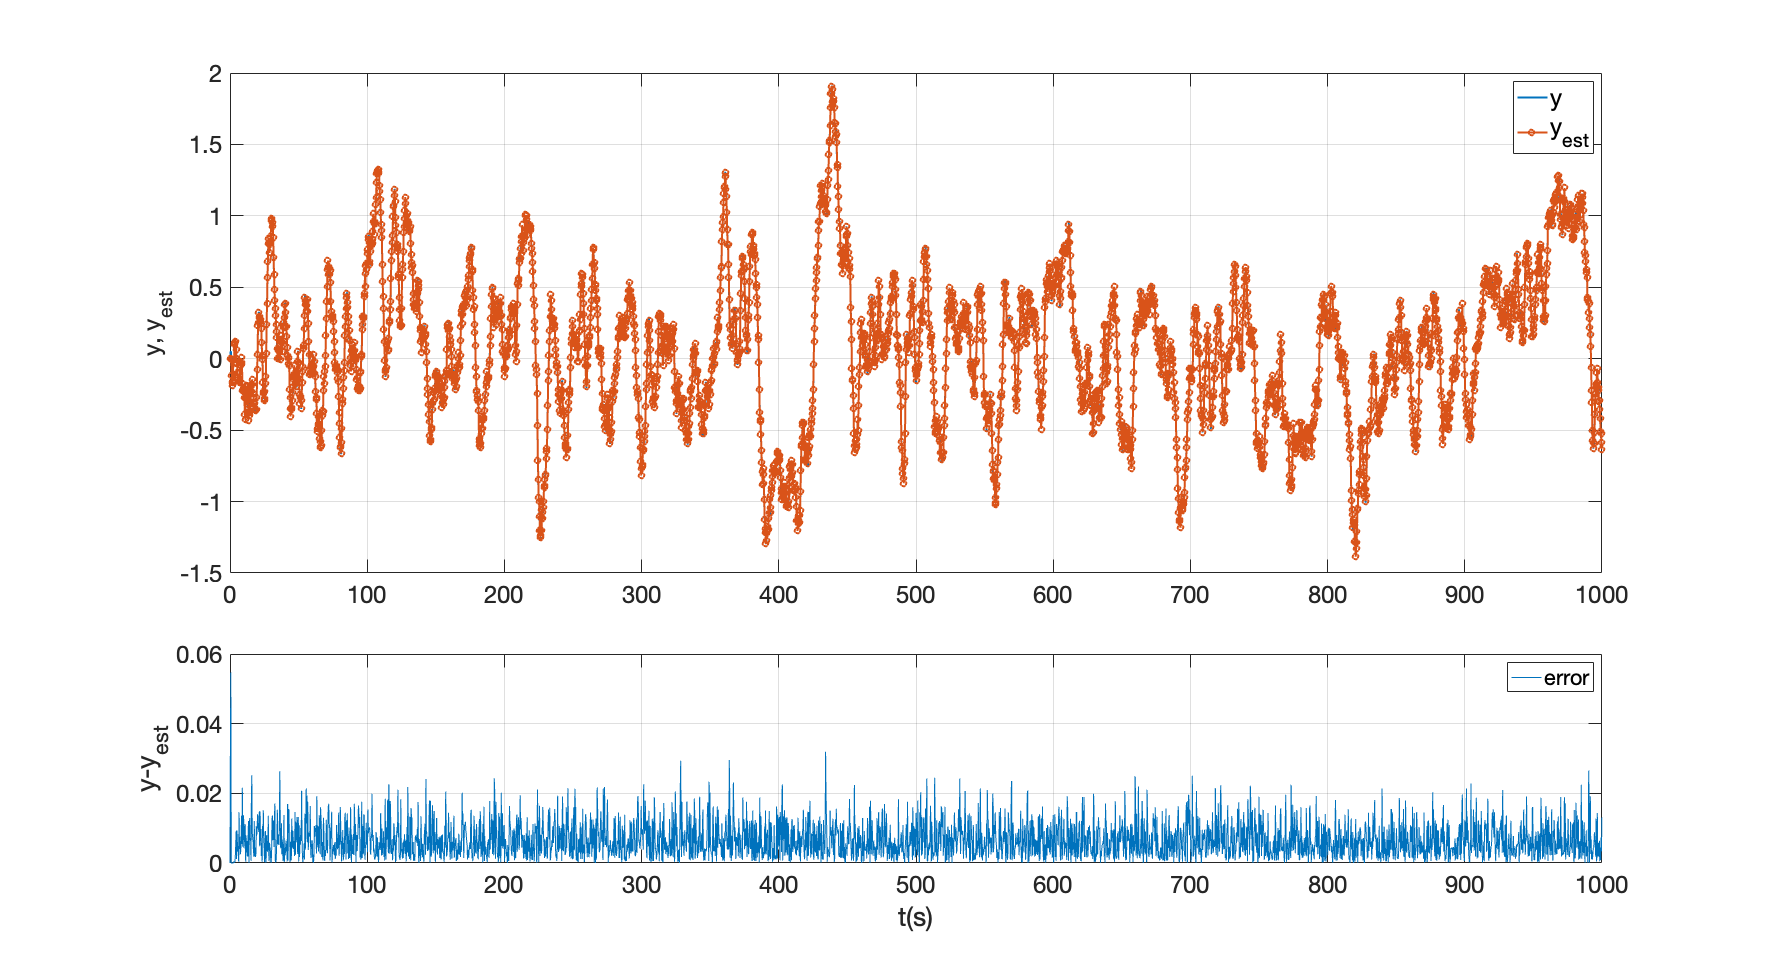
\includegraphics[totalheight=8cm]{images/ELSIColoredNoiseOutput.png}
	\caption{ELS system output comparison for colored noise on output}
	\label{fig:ELSIColoredNoiseOutput}
\end{figure}


\begin{figure}
	\centering
	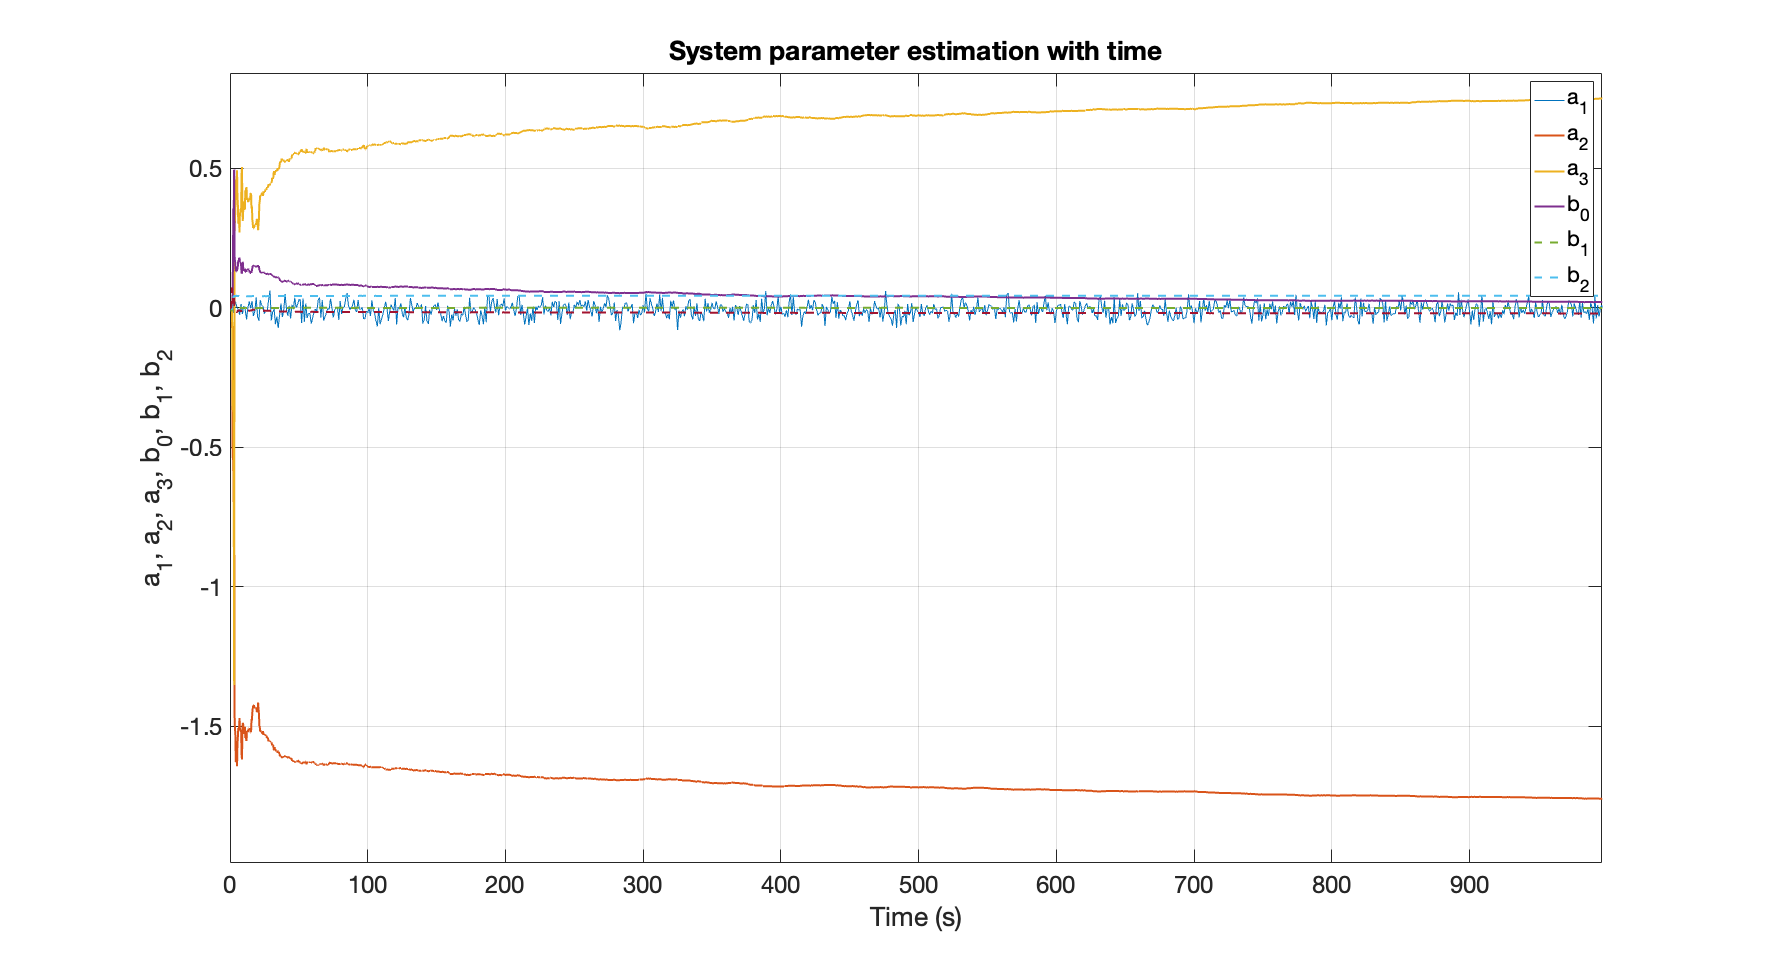
\includegraphics[totalheight=8cm]{images/ELSISystemParam.png}
	\caption{ELS system parameters with colored noise on output}
	\label{fig:ELSISystemParam}
\end{figure}

\begin{figure}
	\centering
	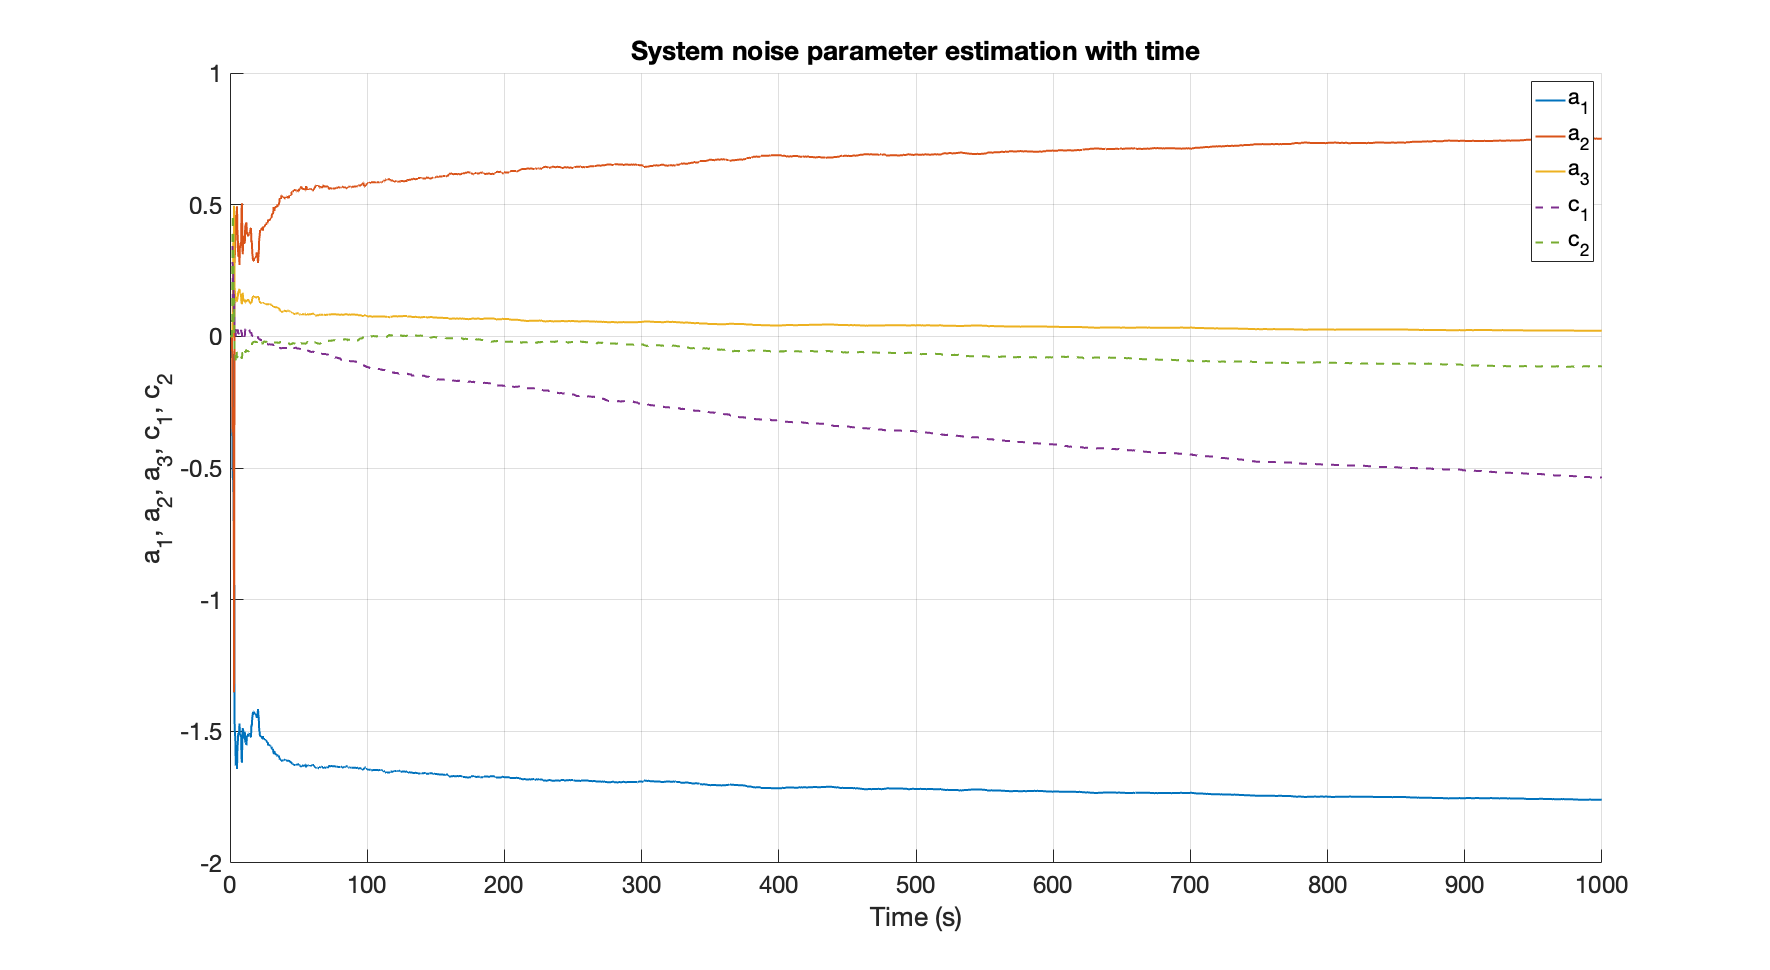
\includegraphics[totalheight=8cm]{images/ELSINoiseParam.png}
	\caption{ELS noise parameters with colored noise on output}
	\label{fig:ELSINoiseParam}
\end{figure}

\begin{equation}
	G(z) =	\frac{ -8.102e-05 z^2 + 0.0436 z - 0.0161}{z^3 - 1.677 z^2 + 0.6355 z + 0.05447}
	\label{eq:ELSITransferFunction}
\end{equation}
